\documentclass[12pt]{article}
\usepackage[english]{babel}
\usepackage[utf8]{inputenc}
\usepackage{amsmath}
\usepackage{graphicx}
\usepackage{float}
\usepackage[colorinlistoftodos]{todonotes}
\usepackage[bottom=1in,top=1in,right=1in,left=1.5in,]{geometry}
\usepackage{setspace}
\doublespacing
\usepackage[lofdepth]{subfig}
\usepackage{graphicx}
\usepackage[nottoc]{tocbibind}
\usepackage{titletoc}
\usepackage[sectionbib]{natbib}
\usepackage{multirow}

\begin{document}
\pagenumbering{gobble}
\

\begin{center}
	\uppercase {Big data analysis of futures: Penalized Regression Splines for trade Volume Prediction and Price Volatility vs trade volume relationship}\\
	\vspace{1in}
	by\\
	Aniver Oluwatobi Bosede\\
	\vspace{1.5in}
	A thesis submitted to Johns Hopkins University in conformity with the requirements for the degree of Master of Science in Engineering\\
	\vspace{.5in}
	Baltimore, Maryland\\
	\vspace{2in}
	\copyright{} 2017 Aniver Oluwatobi Bosede\\
	All Rights Reserved
\end{center}
\newpage
\pagenumbering{roman}
\setcounter{page}{2}

\section*{Abstract}
\addcontentsline{toc}{section}{Abstract}
\newpage

\section*{Acknowledgments}
\addcontentsline{toc}{section}{Acknowledgments}
%remember to acknowledge Naiman and Duncan 
 
\newpage

\tableofcontents
\newpage
\begingroup
\renewcommand\numberline[1]{}
\listoftables
\newpage
\listoffigures
\endgroup
\newpage

\pagenumbering{arabic}	
\setcounter{page}{1}
\section*{Introduction}
\addcontentsline{toc}{section}{Introduction}
%should i indent 1st paragraph? add stuff here about previous methods used such as GARCH, splinsDSC, and NueralNetworks?
Technology has advanced so far that in our society today we are constantly collecting data \cite{economist_10}. This has created the issue of how to feasibly analyze such overwhelming amounts of data \cite{economist_10}. We can then consider how to efficiently store it or how to best carry out statistical computations \cite{zaharia2016apache}. The aforementioned together form the relatively new and evolving field of big data. The research here focuses on the analysis of hundreds of million of rows of futures trading data with the aid of Apache Spark (Spark). 

Spark is a fault-tolerant and general-purpose cluster computing system providing APIs in Java, Scala, Python, and R \cite{meng2016mllib}. Spark was chosen for the analysis over the similarly popular Hadoop MapReduce (MapReduce) because of Spark’s performance advantages as well as its greater computational capabilities \cite{zaharia2010spark}. Not only does Spark cache data resulting in persisted in-memory manipulations \cite{zaharia2012resilient}, it also includes Structured Query Language (SQL) and MLlib, a machine learning library \cite{meng2016mllib}. Conversely, MapReduce only does manipulations via disk reads and thus does not allow for data sharing \cite{zaharia2016apache}. Furthermore for a typical pipeline, external systems would have to be combined with MapReduce to provide querying and machine learning functionality \cite{zaharia2016apache}. In this case, 
A stand alone set up was employed, meaning that analysis was done using a one node cluster setup or one machine. Out of convenience the local file system was used for storage as opposed to a database like Cassandra or HDFS (Hadoop Distributed File System). However, for long term data analysis, it would be worthwhile to invest the time needed to set up a more robust data storage system. 

The futures trading data come from the Chicago Mercantile Exchange (CME) and were collected from May 2, 2016 to November 18, 2016. % only used from about May to September 
Raw data from the CME included extended hours trading and was collected via the Trading Technologies X\_TRADER® API RTD (Real Time Data) server. The server returned raw records with instrument name, maturity, date, time stamp, price, and quantity fields.
The futures were comprised of 21 financial instruments spanning six markets - foreign exchange, metal, energy, index, bond, and agriculture recording roughly a trade every half second. %/home/dnaiman1/findata/big_harvest/Trades_2016_11_18.csv
First, this work uses spline regression to predict the volume of trading for any given day. Volume during a particular time period is taken to mean the number of units traded. A spline regression was chosen due to lack of knowledge regarding the likely non-linear function underlying the response to covariates, in particular time to maturity. Predicting trade volume is of interest because many trading algorithms depend on volume \cite{satish2014predicting}.   Additionally, accurate volume predictions over a given interval allows traders to be more effective \cite{satish2014predicting}. In general, volume prediction increases trading strategy capacity, controls trading risk, and manages slippage \cite{satish2014predicting}.  

Second, the relationship between price volatility and trade volume is explored using standard deviation as a measure of volatility. In particular, volatility vs daily volume and volatility versus hourly volume were plotted to see whether or not the correlation remained the same with the passing of days and hours. It should be noted that unpredictable volume shocks have been known to be more predictive of change in volatility than predictable volume changes \cite{bessembinder1993price}.
%there is evidence suggesting that comparisons between volatility and total volume do not extract all information
This volatility-volume relationship is of importance due to the notion that hedgers are motivated to trade futures to stabilize their future income flows or costs, wherein the volume of their trading is based on their expectation of price variability \cite{foster1995volume}. Likewise, speculators are motivated to trade futures based on expectations of price variability \cite{foster1995volume}. Due to the fact that new information on the market causes agents such as hedgers and speculators to trade until prices reach a revised equilibrium which then changes price and trading volume, we expect a positive correlation between volatility and volume \cite{foster1995volume}. Indeed past research indicates that there is a positive relationship between volume and price volatility \cite{foster1995volume}. This sort of exploration provides information on the efficiency of futures markets which regulators can then use to decide upon market restrictions \cite{foster1995volume}. 
%Talk about what futures are?

\section*{Methods}
\addcontentsline{toc}{section}{Methods}
A cubic regression spline was thought to be appropriate for modeling trade volume. Spline regression derives its name from a draftsman’s spline which is a flexible strip of metal or rubber used to draw curves \cite{harrell2015regression}. Similarly, spline basis functions are piecewise polynomials used in fitting curves which are linear in terms of the basis function. Splines have been used, principally in the physical sciences as well as in biomedicine, to approximate a wide variety of functions \cite{harrell2015regression}. Cubic splines in particular have been found to have nice properties with good ability to fit nonlinear curves. Cubic splines can be made to be smooth at the knots, endpoints of intervals on the x-axis, by forcing the first and second derivatives of the function to agree at the knot \cite{harrell2015regression}.  

Holidays were removed from the raw data. Then the day of the month, day of the week, and hour of the trade were extracted from the time stamp. An aggregation was then done to sum the number of trades per hour for each product, where product is defined as an instrument-maturity pair. There were 148 such products. Aggregation reduced the data from 105 million records to 8826 records. Day, time to maturity, and market fields were created and total trade volume for each day was calculated.

Exploratory analysis was then done on the reduced data set. To ensure that a spline regression was appropriate for modeling trade volume, the first thing done was to create histograms of the trade volumes. One of the assumptions behind regression is that the response conditioned on the predictors is normally distributed. Even if normality fails, regression is feasible, but under normality least squares is optimal. Thus transforming to normality is desirable. The histogram of the raw trade volume was skewed as shown in left of Figure 1. Therefore the volume was Box Cox transformed, after which the data became normal as shown in right of Figure 1.

\begin{figure}[H]
	\begin{center}
	\begin{tabular}{cc}
		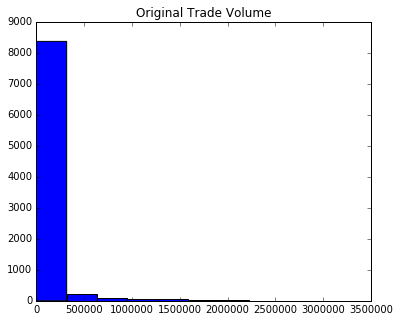
\includegraphics[width=6.5cm]{hist_orig.png}
		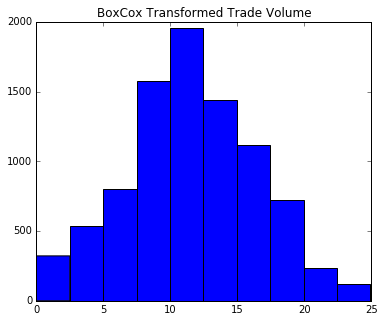
\includegraphics[width=6.25cm]{hist_bc.png}
	\end{tabular}
	\caption{Histograms of before and after Box-Cox transformation of trade volume}
	\label{fig:dum1}
	\end{center}
\end{figure}

There was curiosity regarding how trade volume changed as time passed. Thus a plot of the transformed trade volume versus day (ignoring weekends) was made. Time to maturity was not taken into consideration for  instruments to reduce the number of points plotted. The aggregated trade counts on just instrument reduces the data to 2789 rows. However this resulted in the sums of trades increasing, since all trades of the same instrument in the hour were counted regardless of maturity. Referring to the left plot in Figure 2, the trade volume appears constant across the days with a cluster of high volume trades above 55 which is 797,995 trades. and a cluster of low volume trades below 45 which is 282,640 trades. This implies medium trading is be-

\begin{figure}[H]
	\begin{center}
		\begin{tabular}{cc}
			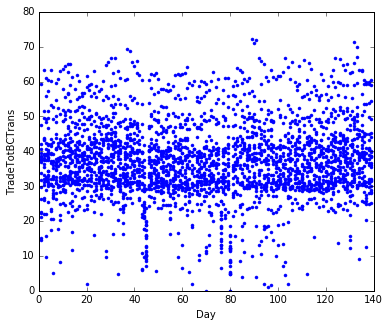
\includegraphics[width=6.5cm]{bc_sample_day.png}
			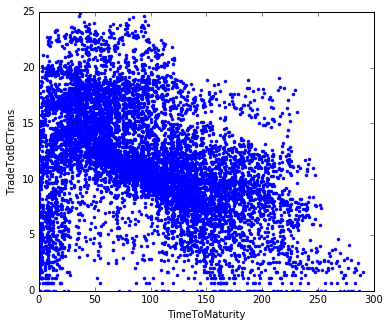
\includegraphics[width=6.5cm]{time_to_mat.png}
		\end{tabular}
		\caption{Plot of trade volume as days pass and as time to maturity gets further.}
		\label{fig:1}
	\end{center}
\end{figure}

\noindent tween 282,640 and 797,995. Also intuitively, it makes sense that less trading occurs far from maturity and near maturity. Far from maturity speculators might not have any information that would move them to purchase a future and most hedgers may only seek to minimize risk in the short term. Then near maturity traders are closing their positions. To confirm this theory a plot was made of the transformed trade volume versus time to maturity, right in Figure 2. Looking at the plot it appears that the data follows intuition. 
 
\begin{figure}[H]
	\begin{center}	
		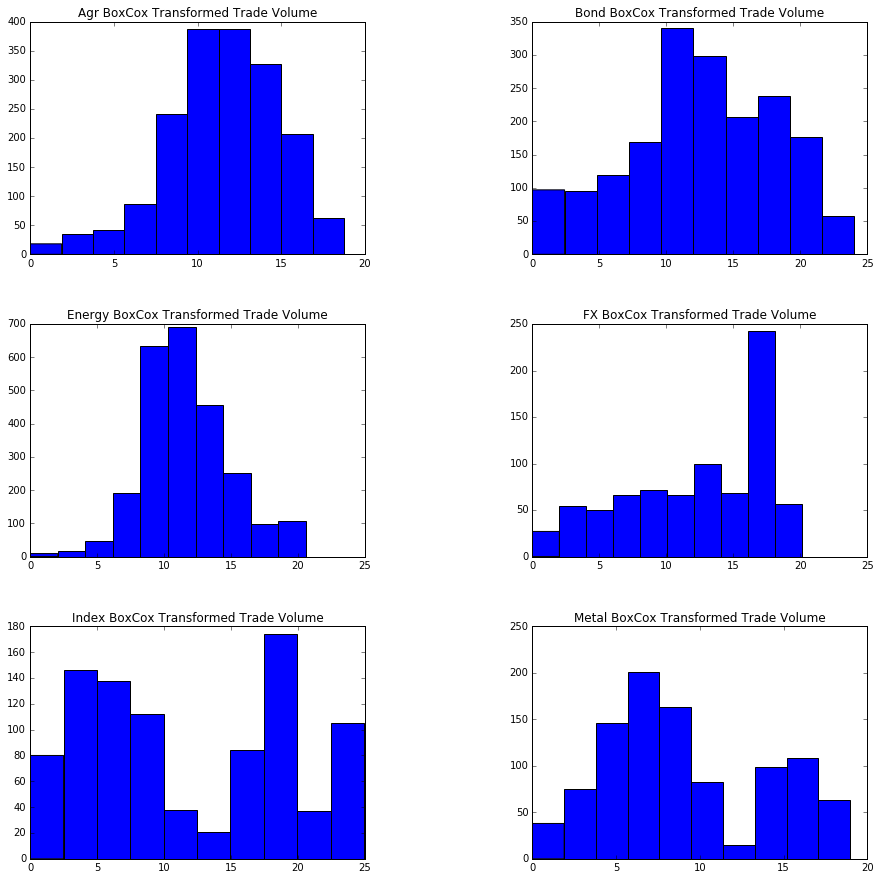
\includegraphics[width=15cm]{types_bc_hist.png}
		\caption{Histograms for instrument types}
		\label{fig:2}
	\end{center}
\end{figure}
Whether it made sense to make one model or several models for each instrument market - foreign exchange, metal, energy, index, bond, and agriculture was also considered. This would mean that each of the markets need to have near normal distributions. In Figure 3 it can be seen that agriculture, bond, and energy are approximately normally distributed after Box-Cox transformation, but foreign exchange, index, and  

\begin{figure}[H]
	\begin{center}	
		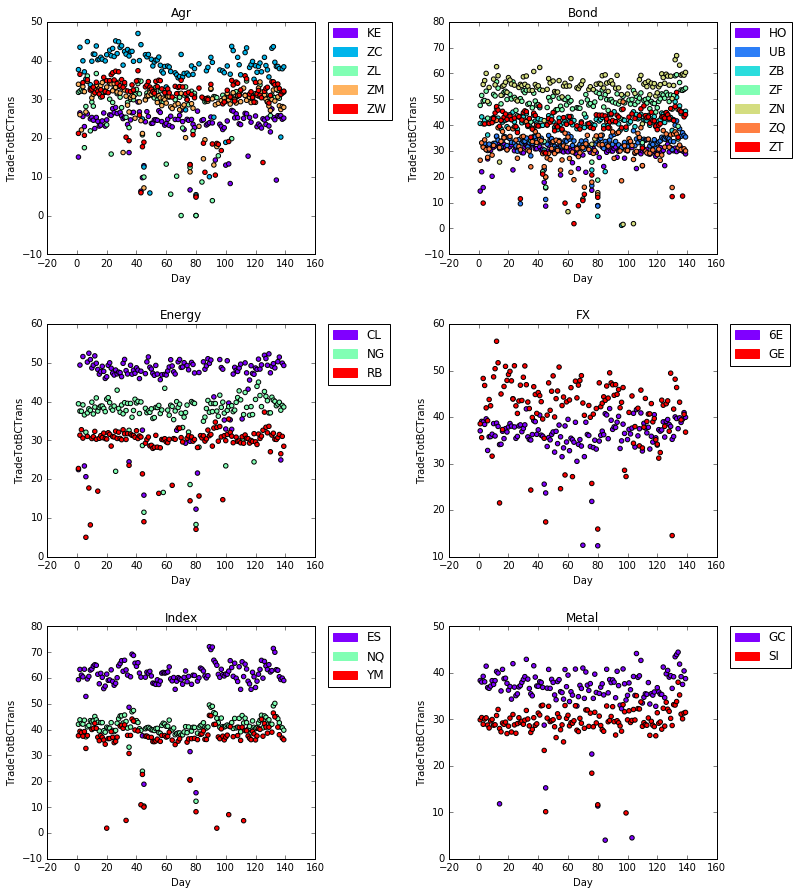
\includegraphics[width=15cm]{agr_scatter_trans.png}
		\caption{Plot of trade volume as days pass for instrument types}
		\label{fig:3}
	\end{center}
\end{figure}

\noindent metal are not. Therefore we expect higher error in the spline model of the latter compared to the former group of instruments. The trend in daily trade volume as time passed was also explored for each instrument market in Figure 4.  These points were then color-coded to understand which instruments comprised the various clusters. It is clear that low volumes of trading occur for metal and agriculture markets compared with bond and index which appear to be more liquid. 

\begin{figure}[H]
	\begin{center}	
		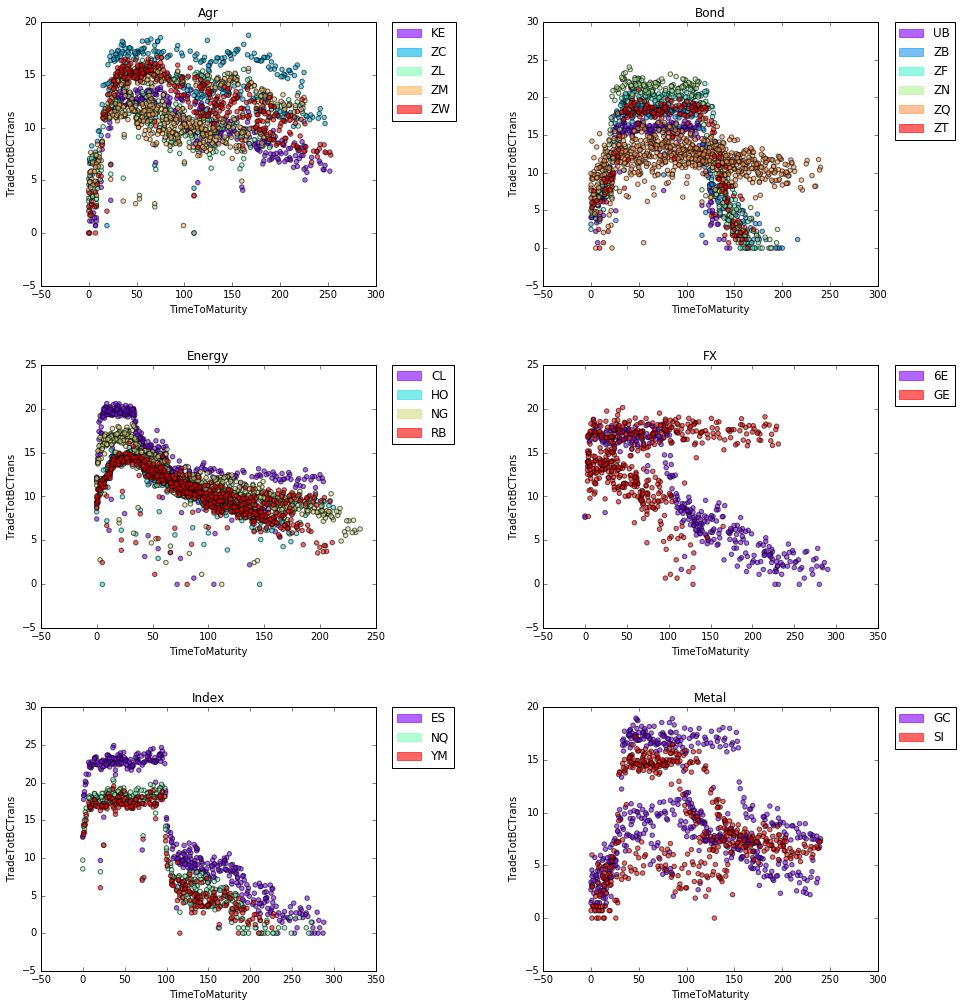
\includegraphics[width=15cm]{types_time_to_mat.png}
		\caption{Plot of trade volume as time to maturity gets further for instrument types}
		\label{fig:4}
	\end{center}
\end{figure}

Finally the trend in daily trade volume as time to maturity increased was visualized for each market in Figure 5. Like the histograms, agriculture, bond, and energy plots follow the general trend of low trade volume far from the maturity and close to maturity, but foreign exchange, index, and metal do not. There is some clustering in the metal and index plots as well which seems in line with the bimodal and trimodal histograms respectively.

%Regression
The above described exploratory analysis deemed spline regression reasonable for trade volume prediction. Thus, both one linear model and multiple linear models paradigms were considered, two versions for each, making four models in total as shown in Table 1. All models under consideration were linear. One model paradigm meant a single model for all markets, whereas the multiple models paradigm meant each market had its own model. Spline variables are denoted by ``s". The models were fit on May to August data and used for forecasting trade volume from September through November. The mean absolute deviation (MAD) was then calculated for each model to compare the errors of forecasted volumes in a robust manner. MAD is defined as: $\displaystyle \sum_{i=1}^{N} \frac{|\hat{Y_i}-Y_i|}{N}$. The models were penalized with an integrated square second derivative cubic spline. This amounted to a natural spline and so generalized cross validation was employed to find an optimal smoothing parameter. The knots were placed at fixed intervals.
%smooth.terms {mgcv}
%smooth.construct.cr.smooth.spec {mgcv}	

\begin{table}[H]
	\caption{Predictors used in models}
	\begin{center}
		\begin{tabular}{ |c|c|c|c| } 
		\hline
		\multicolumn{2}{| c |}{One Linear Model}
		&
		\multicolumn{2}{| c |}{Multiple Linear Models}\\
		\hline
		\hline
		model 1' & model 1 & model 2' & model 2\\
		\hline
		 s(TimeToMaturity) & s(TimeToMaturity) & s(TimeToMaturity) & s(TimeToMaturity) \\ 
		s(DayofMonth) & s(DayofMonth) & s(DayofMonth) & s(DayofMonth) \\ 
		Market & Market & DayOfTheWeek & DayOfTheWeek \\ 
		DayOfTheWeek & DayOfTheWeek &  & Instrument \\
		           & Instrument &  & \\
		\hline
		\end{tabular}
	\end{center}
	\label{tab:dum1}
\end{table}

%Price vol vs trade volume
%reaggregate data for price volitlity
%Really results?
An additional goal of this study was to understand the relationship between price volatility and trade volume. To this end, hourly aggregation similar to that which was done for trade volume was done for price volatility. Volatility was measured using standard deviation. Next each product's hourly price volatility was plotted against its hourly trade volume for the full period over which the data was collected; that is from May to November. Given past research, we expect a positive correlation between price and volume. Consistency of the correlation between price and volume over the days was of interest as well. This was investigated for each product by plotting daily correlations between hourly price volatility and hourly trade volume.
%describe half train on past, half test on future!

\section*{Results}%for trade quantity regression and vol rela
\addcontentsline{toc}{section}{Results}
\begin{figure}[H]
	\begin{center}	
		\caption{Dummy figure}
		\label{fig:5}
	\end{center}
\end{figure}
\begin{figure}[H]
	\begin{center}
		\caption{Dummy figure}
		\label{fig:dum2}
	\end{center}
\end{figure}

\begin{table}[H]
	\caption{Dummy table}
	\begin{center}
		\begin{tabular}{|c|c|}
			
		\end{tabular}
	\end{center}
	\label{tab:dum2}
\end{table}

\section*{Discussion} 
\addcontentsline{toc}{section}{Discussion}

%future work to predict hourly trading, prediction interval can be made more granular

\section*{Appendices} %for code? additional resources?
\addcontentsline{toc}{section}{Appendices}
\newpage

\section*{Bibliography}
\renewcommand{\bibsection}{}
\addcontentsline{toc}{section}{Bibliography}
\bibliographystyle{plain}
\bibliography{example}
\newpage

\section*{Curriculum Vitae}
\addcontentsline{toc}{section}{Curriculum Vitae}

\end{document}